\chapter{Introduction, Finite Automata, Regular Expressions}

The theory of computation begins with a question: What is a computer. The real computer is too complicated to understand, to start with, we use an idealized computer called \textbf{computational model}. 

The simplest model among them is \textbf{finite state machine} or \textbf{finite automaton}.  

\section{Finite Automata}

Finite automata are good models for computers with an extremely limited amount of memory. 

Finite automata and their probabilistic counterpart \textbf{Markov chains} are useful tools when we're attempting to recognize patterns in data. Markov chains have even been used to model and predict price changes in financial markets.

\begin{eg}[Finite Automata Example]
    Here's an example of finite automata:\\
    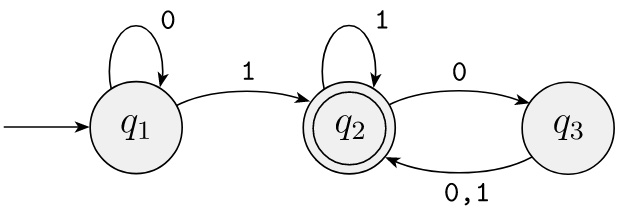
\includegraphics[width=\textwidth]{f1.4.jpg}

    \begin{itemize}
        \item The figure is called \textbf{state diagram} of \(M_1\).
        \item Three \textbf{states}: \(q_1\), \(q_2\) and \(q_3\).
        \item \textbf{Start state}: \(q_1\).   
        \item \textbf{Accept state}: \(q_2\).  
        \item The arrows going from one state to another are called \textbf{transitions}.
    \end{itemize}

    When the automaton receives an input string such as \verb|1101|, it processes that string and produces an output. The output is either \textbf{accept} or \textbf{reject}:
    \begin{enumerate}
        \item Start in state \(q_1\) 
        \item Read \verb|1|, follow transition from \(q_1\) to \(q_2\)  
        \item Read \verb|1|, follow transition from \(q_2\) to \(q_2\)  
        \item Read \verb|0|, follow transition from \(q_2\) to \(q_3\)  
        \item Read \verb|1|, follow transition from \(q_3\) to \(q_2\)  
        \item \(Accept\) because \(M_1\) is in an accept state \(q_2\) at the end of the input   
    \end{enumerate}
\end{eg}

\begin{definition}[Formal Definition of A Finite Automaton]
    A \textbf{finite automaton} is a 5-tuple (\(Q, \Sigma, \delta, q_0, F\)), where
    \begin{enumerate}
        \item \(Q\) is a finite set called \textbf{state} 
        \item \(\Sigma\) is a finite set called the \textbf{alphabet} 
        \item \(\delta: Q \times \Sigma \Rightarrow Q\) is the \textbf{transition function}
        \item \(q_0 \in Q\) is the \textbf{start state}
        \item \(F \subseteq Q\) is the \textbf{set of accept state}         
    \end{enumerate}
\end{definition}

\begin{eg}[Revisit Finite Automata Example]
    Let's revisit the finite automata example \(M_1\) and see from the formal definition perspective: \\
    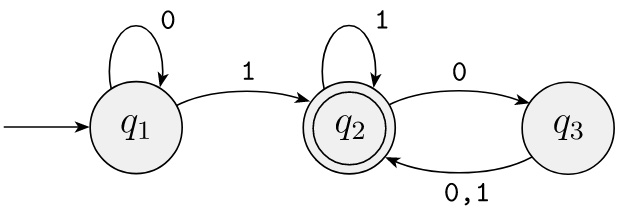
\includegraphics[width=\textwidth]{f1.4.jpg}

    We can describe \(M_1\) formally by writing \(M_1 = (Q, \Sigma, \delta, q_1, F)\), where   
    \begin{enumerate}
        \item \(Q = \{q_1, q_2, q_3\}\)
        \item \(\Sigma = \{ 0, 1 \} \)  
        \item \(\delta\) is described as 
        \begin{table}[H]
            \centering
            \begin{tabular}{c|c|c}
                \toprule
                     & 0 & 1  \\
                \midrule
                   \(q_1\)  & \(q_1\)  & \(q_2\)  \\
                   \(q_2\)  & \(q_3\)  & \(q_2\)  \\
                   \(q_3\)  & \(q_2\)  & \(q_2\)  \\
                \bottomrule
            \end{tabular}
        \end{table}
        \item \(q_1\) is the start state
        \item \(F = \{ q_2 \} \)  
    \end{enumerate}
\end{eg}

If A is the set of all strings that machine \(M\) accepts, we say that A is the \textbf{language of machine M} and write \(L(M) = A\).   
We say that \textbf{M recognizes A} or that \textbf{M accepts A}.     
Here because \(accept\) has different meaning, we use \(recognize\) for the language.  

\begin{remark}
    A machine may accept several strings, but it always recognizes only one language.
    If the machine accepts no strings, it still recognizes one language -- namely, the empty language \(\emptyset\). 
\end{remark}

\begin{eg}[Revisit Finite Automata Example: Language]
    In our example, the language set A can be represented as:

    A = \{\(\omega\)|\(\omega\) contains at least one \verb|1| and an even number of \verb|0|s follow the last \verb|1|\}.

    Then \(L(M_1) = A\), or equivalently, \(M_1\) recognizes \(A\).   
\end{eg}

\begin{eg}
    When describing such a machine:\\
    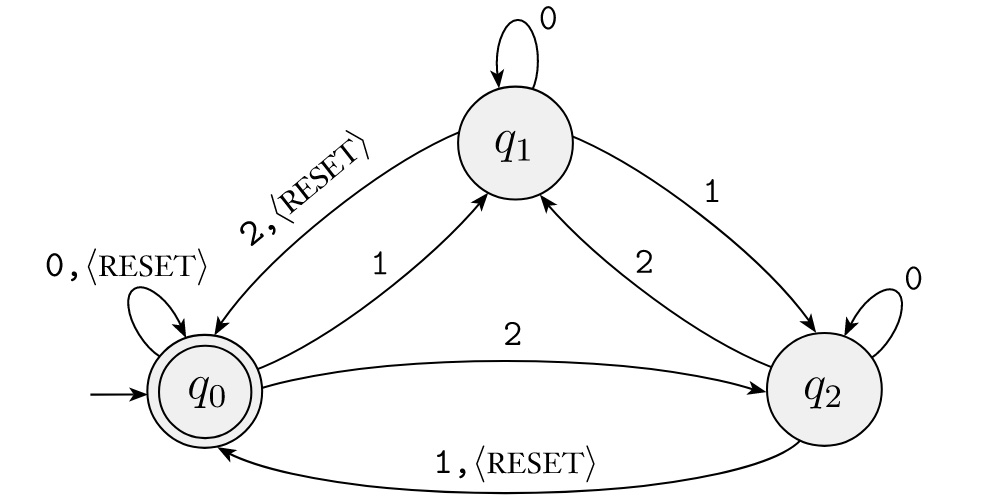
\includegraphics[width=\textwidth]{f1.14.jpg}

    The alphabet \(\Sigma = \{ 1, 2, 3, <RESET> \} \), we treat \(<RESET>\) as a single symbol.  

    The machine keeps a running count of the sum of the numerical input symbols it reads, modulo 3.
    Every time it receives \(<RESET>\) symbol, it resets the count to 0. 
    It accepts if the sum is 0 modulo 3.
\end{eg}

\section{Formal Definition of Computation}

Let \(M = (Q, \Sigma, \delta, q_0, F)\) be a FA and let \(\omega = \omega_1\omega_2\cdots\omega_n\)  be a string where each \(\omega_i\) is a member of alphabet \(\Sigma\).   
Then M \textbf{accepts} \(\omega\) if a sequence of state \(r_0, r_1, \cdots, r_n\) in \(Q\)  exists with three conditions:
\begin{enumerate}
    \item \(r_0 = q_0\) (machine starts at initial state) 
    \item \(\delta(r_i, \omega_{i+1}) = r_{i+1}\)  (machine goes form state to state following the transition function)
    \item \(r_n \in F\) (machine accepts its input if it ends up in an accept state)
\end{enumerate}   

We say that M recognizes language A if \(A = \{ \omega| M accepts \omega \} \) 
\begin{note}
    A is the language, \(\omega\) is the accepted string. 
    A is the set of all instances of \(\omega\). 
    
    We say a machine "accepts" a string, and a machine "recognizes" a language.
\end{note}

\begin{definition}[Regular Language]
    A language is called a \textbf{regular language} if some finite automaton recognizes it. 
\end{definition}

\begin{eg}
    Let B = \{ \( \omega\) | \(\omega\) has even number of 1s \}
    
    B is a regular language.
\end{eg}

\begin{eg}
    Let C = \{ \(\omega\) | \(\omega\) has equal numbers of 0s and 1s \}

    C is \underline{not} a regular language. 
\end{eg}

\section{Regular Expressions}
\subsection{Regular Operations}

\begin{definition}
    Let A and B be languages, we define the regular operations \textbf{union} , \textbf{concatenation} , and \textbf{start} as follows:
    \begin{itemize}
        \item Union: \(A \cup B = \{ x | x \in A || x \in B \} \) 
        \item Concatenation: \(A \circ B = \{ xy | x\in A \& y \in B \} \) 
        \item Star: \(A^* = \{x_1 x_2 \cdots x_k | k \geq 0 \& x_i \in A\}\) 
    \end{itemize}
    
    Notice that \(\epsilon\)(empty language) always belongs to \(A*\).  
\end{definition}

\begin{eg}
    \(\Sigma^*1\) is the language end with 1
\end{eg}

\begin{remark}
    Show finite automata equivalent to regular expressions.
\end{remark}

\subsection{Closure Properties}\label{theorem: clousre properties union}
\begin{theorem}
    The class of regular language is closed under the union operation.

    In other words, if \(A_1\) and \(A_2\) are regular languages, so is \(A_1 \cup A_2\).   
\end{theorem}
\begin{proof}
    Let \(M_1 = \{ Q_1, \Sigma, \delta_1, q_1, F_1 \} \)  recognize \(A_1\). \\
    Let \(M_2 = \{ Q_2, \Sigma, \delta_2, q_2, F_2 \} \)  recognize \(A_2\). 
    (assuming in the same alphabet to make the proof simple)

    Construct \(M = (Q, \Sigma, \delta, q_0, F)\) recognizing \(A_1 \cup A_2\).  

    M should accept input w if either \(M_1\)  or \(M_2\)  accepts w.

    Component of M:
    \begin{itemize}
        \item \(Q = Q_1 \times Q_2\) 
        \item \(q_0 = (q_1, q_2)\) 
        \item \(\delta((q, r), a) = (\delta_1(q, a), \delta(r, a))\) 
        \item \(F = (F_1 \times Q_2) \cup (Q_1 \times F2)\) 
        \item  not \(F = \cancel{F_1 \times F2}\) (this gives intersection!) 
    \end{itemize}
\end{proof}

\begin{eg}[What is close?]
    Positive integers close under addition but not close under subtraction.
\end{eg}

\begin{theorem}\label{theorem: clousre properties concat}
    The class of regular language is closed under the concatenation operation.

    In other words, if \(A_1\) and \(A_2\) are regular languages then so is \(A_1 \circ A_2\).   
\end{theorem}


